\documentclass[a4paper,11pt]{article}
\usepackage{amsmath,amsthm,amsfonts,amssymb,amscd,amstext,vmargin,graphics,graphicx,tabularx,multicol} 
\usepackage[francais]{babel}
\usepackage[utf8]{inputenc}  
\usepackage[T1]{fontenc} 
\usepackage{pstricks-add,tikz,tkz-tab,variations}
\usepackage[autolanguage,np]{numprint} 
\usepackage{calc}

\setmarginsrb{1.5cm}{0.5cm}{1cm}{0.5cm}{0cm}{0cm}{0cm}{0cm} %Gauche, haut, droite, haut
\newcounter{numexo}
\newcommand{\exo}[1]{\stepcounter{numexo}\noindent{\bf Exercice~\thenumexo} : }
\reversemarginpar

\newcommand{\bmul}[1]{\begin{multicols}{#1}}
\newcommand{\emul}{\end{multicols}}

\newcounter{enumtabi}
\newcounter{enumtaba}
\newcommand{\q}{\stepcounter{enumtabi} \theenumtabi.  }
\newcommand{\qa}{\stepcounter{enumtaba} (\alph{enumtaba}) }
\newcommand{\initq}{\setcounter{enumtabi}{0}}
\newcommand{\initqa}{\setcounter{enumtaba}{0}}

\newcommand{\be}{\begin{enumerate}}
\newcommand{\ee}{\end{enumerate}}
\newcommand{\bi}{\begin{itemize}}
\newcommand{\ei}{\end{itemize}}
\newcommand{\bp}{\begin{pspicture*}}
\newcommand{\ep}{\end{pspicture*}}
\newcommand{\bt}{\begin{tabular}}
\newcommand{\et}{\end{tabular}}
\renewcommand{\tabularxcolumn}[1]{>{\centering}m{#1}} %(colonne m{} centrée, au lieu de p par défault) 
\newcommand{\tnl}{\tabularnewline}

\newcommand{\trait}{\noindent \rule{\linewidth}{0.2mm}}
\newcommand{\hs}[1]{\hspace{#1}}
\newcommand{\vs}[1]{\vspace{#1}}

\newcommand{\N}{\mathbb{N}}
\newcommand{\Z}{\mathbb{Z}}
\newcommand{\R}{\mathbb{R}}
\newcommand{\C}{\mathbb{C}}
\newcommand{\Dcal}{\mathcal{D}}
\newcommand{\Ccal}{\mathcal{C}}
\newcommand{\mc}{\mathcal}

\newcommand{\vect}[1]{\overrightarrow{#1}}
\newcommand{\ds}{\displaystyle}
\newcommand{\eq}{\quad \Leftrightarrow \quad}
\newcommand{\vecti}{\vec{\imath}}
\newcommand{\vectj}{\vec{\jmath}}
\newcommand{\Oij}{(O;\vec{\imath}, \vec{\jmath})}
\newcommand{\OIJ}{(O;I,J)}


\newcommand{\reponse}[1][1]{%
\multido{}{#1}{\makebox[\linewidth]{\rule[0pt]{0pt}{20pt}\dotfill}
}}

\newcommand{\titre}[5] 
% #1: titre #2: haut gauche #3: bas gauche #4: haut droite #5: bas droite
{
\noindent #2 \hfill #4 \\
#3 \hfill #5

\vspace{-1.6cm}

\begin{center}\rule{6cm}{0.5mm}\end{center}
\vspace{0.2cm}
\begin{center}{\large{\textbf{#1}}}\end{center}
\begin{center}\rule{6cm}{0.5mm}\end{center}
}



\begin{document}
\pagestyle{empty}
\titre{Séance d'AP 6  : Optimisation}{}{}{3ème}{}

Avec une corde de longueur 11 m étendue sur le sol, on fabrique un rectangle.\\
On désigne par $x$ la longueur d'un côté de ce rectangle.\\

\begin{center}
\includegraphics[scale=0.9]{optimisation1.eps} 
\end{center}

\textbf{\underline{Problème :} On cherche avec cette corde à connaître la longueur du rectangle, la valeur de $x$, pour laquelle l'aire du rectangle sera la plus grande possible.}\\

\vspace*{0.7cm}

\textbf{PARTIE A } - Première approche\\

 \q Quelles sont les dimensions du rectangle lorsque x = 1 m ? Faire un schéma pour illustrer si besoin. Calculer ensuite l'aire du rectangle dans ce cas.\\
 
\q Mêmes questions pour x = 2 m.\\

\q A votre avis, quel est la longueur du rectangle pour que l'aire soit la plus grande possible ?\\


\vspace*{0.7cm}


\textbf{PARTIE B } - Modélisation avec une fonction\\

 \initq \q Exprimer les dimensions du rectangle en fonction de x.\\
 
\q Soit A  la fonction qui a $x$ associe l'aire du rectangle.\\
Démontrer que l'aire A du rectangle s'exprime, en fonction de $x$, par la formule : $A(x) = 5,5x - x^{2}$.\\

  \q On cherche la valeur de $x$ pour laquelle l'aire A du rectangle est la plus grande possible.\\

\qa Pour les différentes valeurs de $x$ données dans le tableau, calculer l'aire $A(x)$ du rectangle et compléter le tableau.\\

\renewcommand{\arraystretch}{2}

\begin{center}
 \begin{tabular}{|c|c|c|c|c|c|c|c|c|}
\hline 
$x$ (en m) & \hspace*{0.2cm} 1 \hspace*{0.2cm}& \hspace*{0.2cm}1,4 \hspace*{0.2cm}& \hspace*{0.2cm}1,8 \hspace*{0.2cm}& \hspace*{0.2cm}2,2 \hspace*{0.2cm}& \hspace*{0.2cm}2,6\hspace*{0.2cm} &\hspace*{0.2cm} 3 \hspace*{0.2cm}& \hspace*{0.2cm}3,4 \hspace*{0.2cm}&\hspace*{0.2cm} 3,8 \hspace*{0.2cm}\\ 
\hline 
$A(x)$ (en . . . ) & 4,5 &  &  &  &  &  &  & \\ 
\hline 
\end{tabular}
 \end{center} 

\vspace*{0.3cm}

\qa Pour quelle valeur de $x$, l'aire A du rectangle semble-t-elle la plus grande ?\\


 \q \initqa \qa Dans un repère, placer tous les points dont les coordonnées (x ; A(x)) sont données dans le tableau précédent.\\

\qa Estimer graphiquement l'aire maximale du rectangle et donner la valeur de $x$ pour laquelle cette aire est la plus grande. \\
Comparer votre réponse à la réponse de la question 3) b). Que constatez-vous?



\end{document}
